\documentclass[12pt]{article}
\usepackage[margin=2.5cm]{geometry}
\usepackage{enumerate}
\usepackage{amsfonts}
\usepackage{amsmath}
\usepackage{fancyhdr}
\usepackage{amsmath}
\usepackage{amssymb}
\usepackage{amsthm}
\usepackage{mdframed}
\usepackage{graphicx}
\usepackage{subcaption}
\usepackage{adjustbox}
\usepackage{listings}
\usepackage{xcolor}
\usepackage{booktabs}
\usepackage[utf]{kotex}

\definecolor{codegreen}{rgb}{0,0.6,0}
\definecolor{codegray}{rgb}{0.5,0.5,0.5}
\definecolor{codepurple}{rgb}{0.58,0,0.82}
\definecolor{backcolour}{rgb}{0.95,0.95,0.92}

\lstdefinestyle{mystyle}{
    backgroundcolor=\color{backcolour},
    commentstyle=\color{codegreen},
    keywordstyle=\color{magenta},
    numberstyle=\tiny\color{codegray},
    stringstyle=\color{codepurple},
    basicstyle=\ttfamily\footnotesize,
    breakatwhitespace=false,
    breaklines=true,
    captionpos=b,
    keepspaces=true,
    numbers=left,
    numbersep=5pt,
    showspaces=false,
    showstringspaces=false,
    showtabs=false,
    tabsize=1
}

\lstset{style=mystyle}

\begin{document}
\title{CSC236 Assignment 1}
\author{Hyungmo Gu}
\maketitle

\section*{Question 1}
\begin{enumerate}[a.]
    \item

    Yes. We can prove $P(235)$ follows from $P(234)$.

    \bigskip

    \begin{proof}
    Let $b$ be the bipartite graph with 235 vertices where
    117 vertices are in one partition and 118 vertices in
    the other partition (Note this is the configuration where maximum number of edges form).

    \bigskip

    The bipartite graph with 117 vertices on both sides of partition has
    $\frac{234^2}{4}$ edges, and the assumption tells us this is the maximum number of edges the
    bipartite graph could form.

    \bigskip

    Since we know $b$ has 117 more edges than the bipartite graph with 117 vertices on
    both sides, using these facts, we can conclude the upper bound number of edges for the bipartite
    graph with 235 vertices is

    \begin{align}
        \frac{234^2}{4} + 117 &= \frac{234^2}{4} + \frac{4 \cdot 117}{4}\\
        &= \frac{234^2 + 2 \cdot 234}{4}\\
        &\leq \frac{234^2 + 2 \cdot 234 + 1}{4}\\
        &= \frac{(234+1)^2}{4}\\
        &= \frac{(235)^2}{4}
    \end{align}

    \end{proof}

    \bigskip

    \begin{mdframed}
        \underline{\textbf{Attempt \#2:}}

        \bigskip

        Assume $P(234)$. That is, every bipartite graph on 234 vertices has no more
        than $\frac{234^2}{4}$ edges.

        \bigskip

        We need to prove $P(235)$ follows. That is, every bipartite graph on 235
        vertices has no more than $\frac{235^2}{4}$ edges.

        \bigskip

        Let $b$ be the bipartite graph with 235 vertices. Let $b'$ be the bipartite
        graph with a vertex removed from the larger of two partitions in $b$ along with its edges.

        \bigskip

        Since we know the maximum number of edges occur in $b'$ when there are
        117 vertices in both sides of the partitions, and since we know the edges
        of removed vertex forms edges with partition with bigger number of vertices,
        we can conclude the removed vertex forms at most 117 edges.

        \bigskip

        Since the assumption tells us $b'$ has at most $\frac{234^2}{4}$ edges,
        we can conclude the upper bound number of edges for the bipartite
        graph with 235 vertices is


        \begin{align}
            \frac{234^2}{4} + 117 &= \frac{234^2}{4} + \frac{4 \cdot 117}{4}\\
            &= \frac{234^2 + 2 \cdot 234}{4}\\
            &\leq \frac{234^2 + 2 \cdot 234 + 1}{4}\\
            &= \frac{(234+1)^2}{4}\\
            &= \frac{(235)^2}{4}
        \end{align}

        \bigskip

        So $P(235)$ follows.

    \end{mdframed}

    \bigskip

    \underline{\textbf{Notes:}}

    \bigskip

    \begin{itemize}
        \item I have a stuck feeling as to how I can formulate this kind of proof.
        \item 5+ hours spent on this problem
        \item I feel I wronged the proof by using existential quantifier
        \item Noticed professor generalized his statement instead of using bipartite
        with $x$ number of vertices in one partition and $y$ vertices in other partition
        example

        \begin{center}
        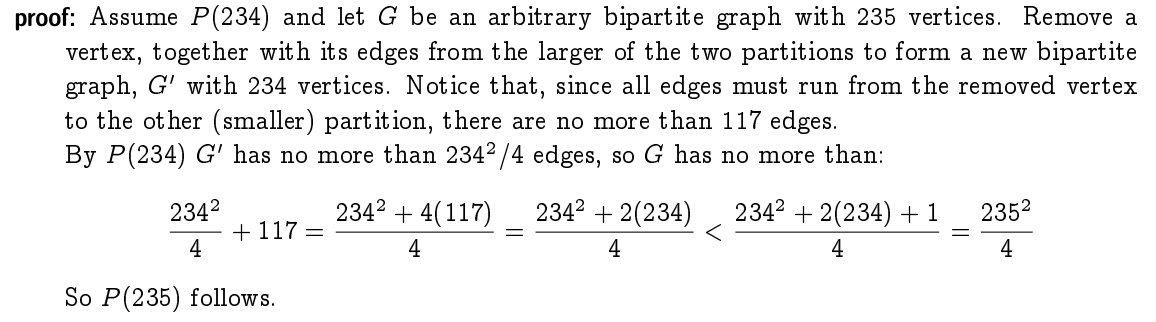
\includegraphics[width=0.8\linewidth]{images/assignment_1_q1a_note.png}
        \end{center}
    \end{itemize}

    % \bigskip

    % \begin{mdframed}
    %     \underline{\textbf{Rough Work:}}

    %     Assume $P(234)$. That is, every bipartite graph on 234 vertices has no more
    %     than $\frac{234^2}{4}$ edges.

    %     \bigskip

    %     We need to prove $P(235)$ follows. That is, every bipartite graph on 235
    %     vertices has no more than $\frac{235^2}{4}$ edges.

    %     \begin{enumerate}[1.]
    %         \item Find the configuration where bipartite graph on 235 vertices form most number of edges in
    %         terms of bipartite graph on 234 vertices.

    %         \begin{mdframed}
    %         Let $b$ be the bipartite graph with 235 vertices where
    %         117 vertices are in one partition and 118 vertices in
    %         the other partition (Note this is the configuration where maximum number of edges form).

    %         \end{mdframed}

    %         \item Show that $\frac{235^2}{4}$ is the most number of edges bipartite graph on 235
    %         vertices could form.

    %         \begin{mdframed}
    %         The bipartite graph with 117 vertices on both sides of partition has
    %         $\frac{234^2}{4}$ edges, and the assumption tells us this is the maximum number of edges the
    %         bipartite graph could form.

    %         \bigskip

    %         Since we know $b$ has 117 more edges than the bipartite graph with 117 vertices on
    %         both sides, using these facts, we can conclude the upper bound number of edges for the bipartite
    %         graph with 235 vertices is

    %         \begin{align}
    %             \frac{234^2}{4} + 117 &= \frac{234^2}{4} + \frac{4 \cdot 117}{4}\\
    %             &= \frac{234^2 + 2 \cdot 234}{4}\\
    %             &\leq \frac{234^2 + 2 \cdot 234 + 1}{4}\\
    %             &= \frac{(234+1)^2}{4}\\
    %             &= \frac{(235)^2}{4}
    %         \end{align}

    %         \bigskip
    %         \end{mdframed}
    %     \end{enumerate}

    % \end{mdframed}

    \item

    No. $P(236)$ doesn't follow from $P(235)$.

    \bigskip

    \begin{proof}
        Assume $P(235)$. That is, every bipartite graph with 235 vertices has no
        more than $\frac{235^2}{4}$ edges.

        \bigskip

        We need to show $P(236)$ doesn't follow. That is, there is a bipartite graph
        $b$ with 236 vertices that has more than $\frac{236^2}{4}$ edges.

        \bigskip

        Let $b$ be bipartite graph with 118 vertices in $V_1$ and 118 vertices in
        $V_2$ (Notice that this forms the most number of edges).

        \bigskip

        The assumption tells us that every bipartite graph with 235 vertices
        has $\frac{235^2}{4}$ edges.

        \bigskip

        Since we know that by removing a vertex with 118 edges from either one
        of the partition results in bipartite graph with 235 vertices, using
        above fact, we can write that $b$ has

        \setcounter{equation}{0}
        \begin{align}
            \frac{235^2}{4} + 118 = 13924.25
        \end{align}

        edges.

        \bigskip

        Since $\frac{236^2}{4} = 13924.0$, we can conclude $P(236)$ doesn't follow.

    \end{proof}

    \bigskip

    \underline{\textbf{Notes:}}

    \begin{itemize}
        \item Noticed that professor tried to show the bipartite graph with
        234 vertices with 117 vertices in $V_1$ and 117 vertices in $V_2$ is the
        one and the only bipartite graph with 234 vertices that form the most number of edges.
    \end{itemize}

    % \bigskip

    % \begin{mdframed}
    %     \underline{\textbf{Rough Work:}}

    %     \bigskip

    %     Assume $P(235)$. That is, every bipartite graph with 235 vertices has no
    %     more than $\frac{235^2}{4}$ edges.

    %     \bigskip

    %     We need to show $P(236)$ doesn't follow. That is, there is a bipartite graph
    %     $b$ with 236 vertices that has more than $\frac{236^2}{4}$ edges.

    %     \bigskip

    %     Let $b$ be bipartite graph with 118 vertices in $V_1$ and 118 vertices in
    %     $V_2$ (Notice that this forms the most number of edges).

    %     \begin{enumerate}[1.]

    %         \item Show that this is 118 edges more than $\frac{235^2}{4}$.

    %         \begin{mdframed}

    %         The assumption tells us that every bipartite graph with 235 vertices
    %         has $\frac{235^2}{4}$ edges.

    %         \bigskip

    %         Since we know that by removing a vertex with 118 edges from either one
    %         of the partition results in bipartite graph with 235 vertices, using
    %         above fact, we can write that $b$ has

    %         \begin{align}
    %             \frac{235^2}{4} + 118 = 13924.25
    %         \end{align}

    %         edges.

    %         \end{mdframed}

    %         \item Conclude this choice of $b$ has more than $\frac{236^2}{4}$ edges.
    %         \begin{mdframed}
    %         Since $\frac{236^2}{4} = 13924.0$, we can conclude $P(236)$ doesn't follow.
    %         \end{mdframed}
    %     \end{enumerate}

    %     \bigskip

    %     \begin{mdframed}
    %         Assume $P(235)$. That is, every bipartite graph with 235 vertices has no
    %         more than $\frac{235^2}{4}$ edges.

    %         \bigskip

    %         We need to show $P(236)$ doesn't follow. That is, there is a bipartite graph
    %         $b$ with 236 vertices that has more than $\frac{236^2}{4}$ edges.

    %         \bigskip

    %         Let $b$ be bipartite graph with 118 vertices in $V_1$ and 118 vertices in
    %         $V_2$ (Notice that this forms the most number of edges).

    %         \bigskip

    %         The assumption tells us that every bipartite graph with 235 vertices
    %         has $\frac{235^2}{4}$ edges.

    %         \bigskip

    %         Since we know that by removing a vertex with 118 edges from either one
    %         of the partition results in bipartite graph with 235 vertices, using
    %         above fact, we can write that $b$ has

    %         \begin{align}
    %             \frac{235^2}{4} + 118 = 13924.25
    %         \end{align}

    %         edges.

    %         \bigskip

    %         Since $\frac{236^2}{4} = 13924.0$, we can conclude $P(236)$ doesn't follow.
    %     \end{mdframed}

    % \end{mdframed}

    \item

    \bigskip

    \begin{proof}
        For convenience, define

        \begin{align*}
        & H(n'):\:\text{Every bipartite graph with $n'$ vertices has no more than
        $\frac{n'^2-1}{4}$ edges}\\
        & \text{when $n'$ is odd, or $\frac{n'^2}{4}$ edges when $n'$ is even.}
        \end{align*}

        \bigskip

        I must prove $\forall n \in \mathbb{N}$, $H(n)$.

        \bigskip

        \underline{\textbf{Base Case ($n = 0$):}}

        \bigskip

        The definition of edge tells us that to form, it requires a pair of two
        distinct vertices.

        \bigskip

        Since the graph has 0 vertices, we can conclude no edge can be
        formed.

        \bigskip

        \underline{\textbf{Inductive Step:}}

        \bigskip

        Let $n \in \mathbb{N}$. And assume $H(n)$.

        \bigskip

        We must prove that $H(n+1)$ is true. There are two cases: $n+1$ is odd, or
        $n+1$ is even.

        \bigskip

        \textbf{Case 1 ($n+1$ is even):}

        \bigskip

        Assume $n+1$ is even. That is, $\exists k \in \mathbb{Z}$ such that
        $n+1 = 2k$.

        \bigskip

        Let $b$ be an arbitrary bipartite graph with $n+1$ vertices. Let
        $v$ be the vertex in larger of two partitions.

        \bigskip

        We must prove $H(n+1)$ is true. That is, every bipartite graph
        with $n+1$ vertices has no more than $\frac{(n+1)^2}{4} = \frac{(2k)^2}{4}$
        edges.

        \bigskip

        First, we need to show $k$ is the most number of edges $v$
        could have in $b$.

        \bigskip

        The definition of bipartite graph tells us the edges of vertex
        $v$ runs from $v$ to each vertex in the smaller partition.

        \bigskip

        Since we know the smaller partition has at most $\frac{n+1}{2} = k$,
        vertices, we can write the vertex $v$ has no more than $k$ edges.

        \bigskip

        Second, we need to show the bipartite graph with $n$ vertices has
        at most $\frac{4k^2-4k}{4}$ edges.

        \bigskip

        The assumption tells us every bipartite graph with $n'$ vertices
        has no more than $\frac{n'^2-1}{4}$ edges when $n'$ is odd, or
        $\frac{n'^2}{4}$ edges when $n'$ is even.

        \bigskip

        Since we know $n = 2k - 1$ is odd, we can write the bipartite
        graph with $n$ vertices has no more than

        \begin{align}
            \frac{n^2-1}{4} &= \frac{(2k-1)^2-1}{4}\\
            &= \frac{4k^2-4k+1-1}{4}\\
            &= \frac{4k^2-4k}{4}
        \end{align}

        edges.

        \bigskip

        Finally, by combining the two together, and using the fact $k \geq 1$
        (note this is required for $n$ to stay positive), we can
        conclude the bipartite graph has no more than

        \begin{align}
            \frac{n^2-1}{4} + k &=\frac{4k^2-4k}{4} + k\\
            &= \frac{4k^2-4k}{4} + \frac{4k}{4}\\
            &= \frac{4k^2}{4}\\
            &= \frac{(2k)^2}{4}\\
            &= \frac{(2k)^2}{4}\\
            &= \frac{(n+1)^2}{4}
        \end{align}

        edges.

        \bigskip

        \textbf{Case 2 ($n+1$ is odd):}

        \bigskip

        Assume $n+1$ is odd. That is, $\exists k \in \mathbb{Z}$ such that
        $n+1 = 2k-1$.

        \bigskip

        Let $b$ be an arbitrary bipartite graph with $n+1$ vertices. Let
        $v$ be the vertex in larger of two partitions.

        \bigskip

        We must prove $H(n+1)$ is true. That is, every bipartite graph
        with $n+1$ vertices has no more than $\frac{(n+1)^2-1}{4} = \frac{n(n+2)}{4} = \frac{2k(2k-2)}{4}$
        edges.

        \bigskip

        First, we need to show $k-1$ is the most number of edges $v$
        could have in $b$.

        \bigskip

        The definition of bipartite graph tells us the edges of vertex
        $v$ runs from $v$ to each vertex in the smaller partition.

        \bigskip

        Since we know the smaller partition has at most $\frac{n}{2} = \frac{2k-2}{2} = k - 1$,
        vertices, we can write the vertex $v$ has no more than $k-1$ edges.

        \bigskip

        Second, we need to show the bipartite graph with $n$ vertices has
        at most $\frac{(2k-2)^2}{4}$ edges

        \bigskip

        The assumption tells us every bipartite graph with $n'$ vertices
        has no more than $\frac{n'^2-1}{4}$ edges when $n'$ is odd, or
        $\frac{n'^2}{4}$ edges when $n'$ is even.

        \bigskip

        Since we know $n = 2k - 2$ is even, we can write the bipartite
        graph with $n$ vertices has no more than

        \begin{align}
            \frac{n^2}{4} &= \frac{(2k-2)^2}{4}
        \end{align}

        edges.

        \bigskip

        Finally, by combining the two together, we can conclude the
        bipartite graph has no more than

        \begin{align}
            \frac{n^2}{4} + k-1 &= \frac{(2k-2)^2}{4} + k-1\\
            &= \frac{(2k-2)^2}{4} + \frac{4k-4}{4}\\
            &= \frac{4k^2-8k+4}{4} + \frac{4k-4}{4}\\
            &= \frac{2k(k-2)}{4}\\
            &= \frac{(n+2) \cdot n}{4}\\
            &= \frac{(n+1)^2 - 1}{4}
        \end{align}

        edges.

    \end{proof}

    \newpage

    \underline{\textbf{Notes:}}

    \begin{itemize}
        \item Learned the line `Remove a vertex, together with its edges from the larger
        of the two partitions to form a new bipartite graph ... Notice that,
        since all edges must run from the removed vertex to other smaller partition,
        there are no more than...' means the following

        \begin{center}
        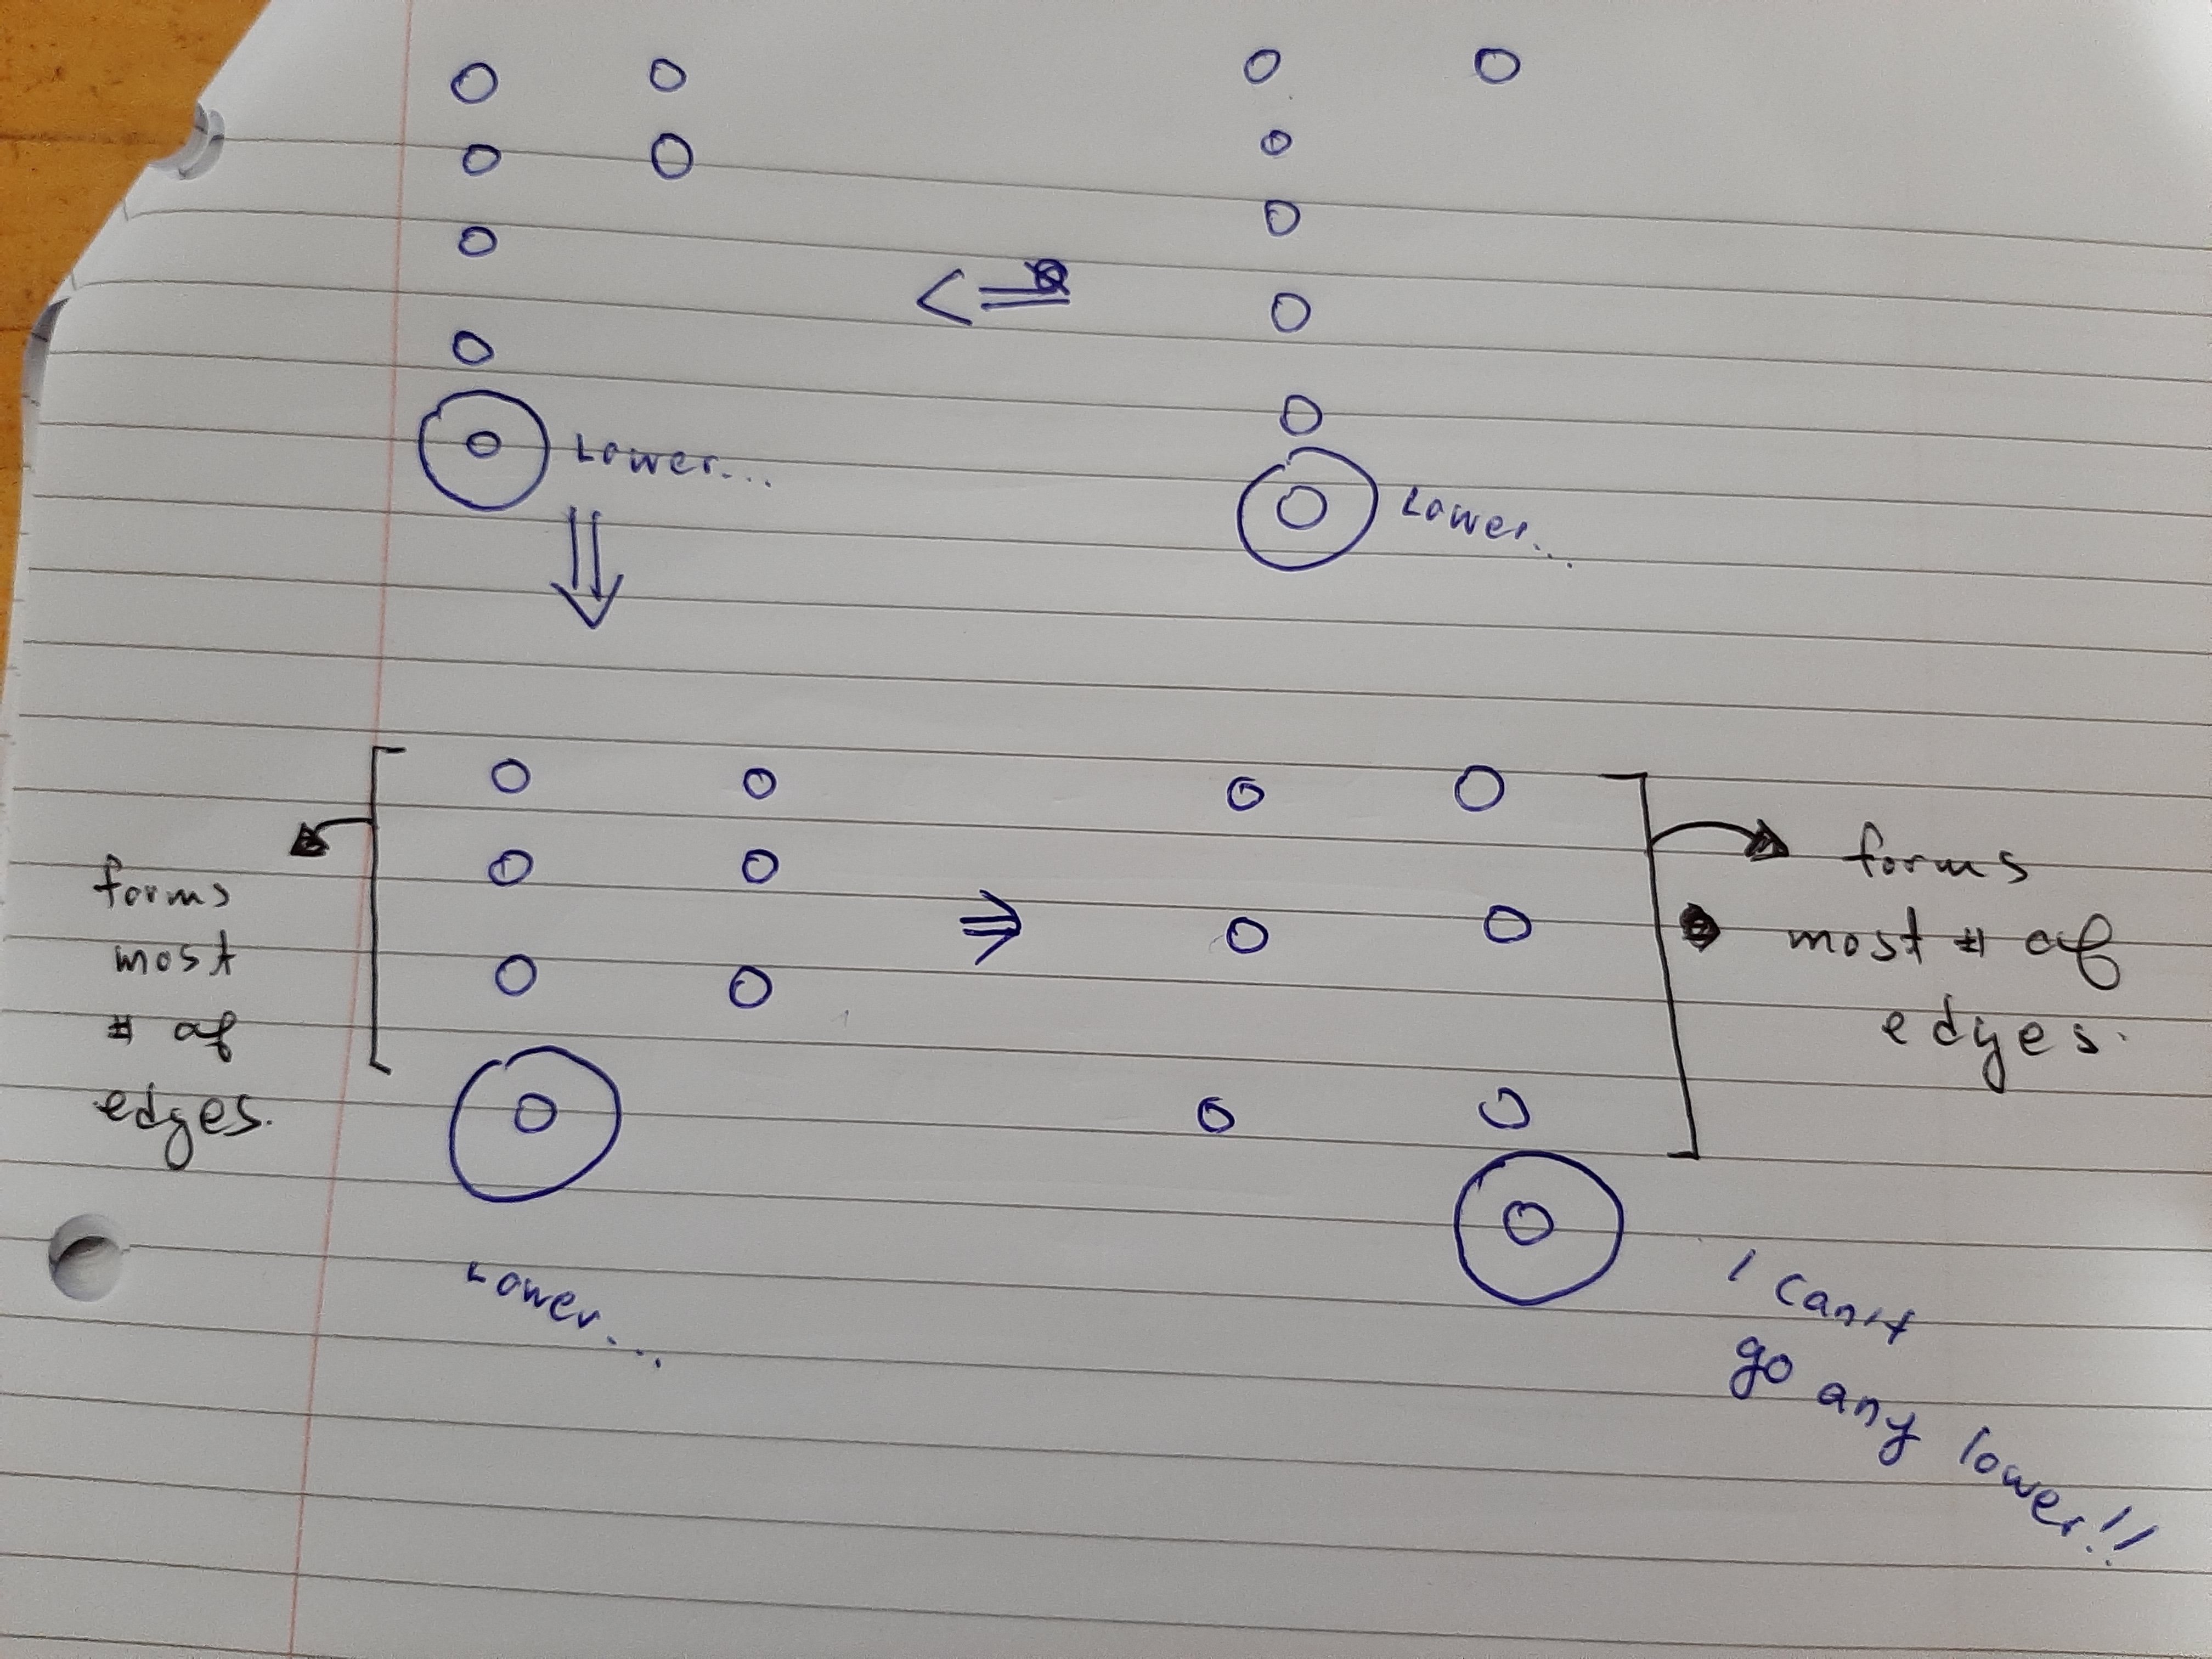
\includegraphics[width=0.8\linewidth]{images/assignment_1_q1c_note.jpg}
        \end{center}

        \item This was tricky. And the trick is sneaky :).
    \end{itemize}


    % \begin{mdframed}
    %     \underline{\textbf{Rough Work:}}

    %     \bigskip

    %     For convenience, define

    %     \begin{align*}
    %     & H(n'):\:\text{Every bipartite graph with $n'$ vertices has no more than
    %     $\frac{n'^2-1}{4}$ edges}\\
    %     & \text{when $n'$ is odd, or $\frac{n'^2}{4}$ edges when $n'$ is even.}
    %     \end{align*}

    %     \bigskip

    %     I must prove $\forall n \in \mathbb{N}$, $H(n)$.

    %     \bigskip

    %     \begin{enumerate}[1.]
    %         \item Base Case ($n = 0$)

    %         \bigskip

    %         We need to verify $H(0)$. That is, every bipartite graph with 0 vertices
    %         has no more than 0 edges.

    %         \bigskip

    %         \begin{itemize}
    %             \item State that bipartite graph with 0 vertices has 0 edge, and conclude $H(n)$ is verified.

    %             \begin{mdframed}
    %             The definition of edge tells us that to form, it requires a pair of two
    %             distinct vertices.

    %             \bigskip

    %             Since the graph has 0 vertices, we can conclude no edge can be
    %             formed.
    %             \end{mdframed}
    %         \end{itemize}

    %         \item Inductive Step

    %         \bigskip

    %         Let $n \in \mathbb{N}$. And assume $H(n)$.

    %         \bigskip

    %         We must prove that $H(n+1)$ is true. There are two cases: $n+1$ is odd, or
    %         $n+1$ is even.

    %         \bigskip

    %         \begin{enumerate}[1.]
    %             \item Case 1 ($n+1$ is even)

    %             \bigskip

    %             Assume $n+1$ is even. That is, $\exists k \in \mathbb{Z}$ such that
    %             $n+1 = 2k$. Assume $H(n)$.

    %             \bigskip

    %             Let $b$ be an arbitrary bipartite graph with $n+1$ vertices. Let
    %             $v$ be the vertex in larger of two partitions.

    %             \bigskip

    %             We must prove $H(n+1)$ is true. That is, every bipartite graph
    %             with $n+1$ vertices has no more than $\frac{(n+1)^2}{4} = \frac{(2k)^2}{4}$
    %             edges.

    %             \bigskip

    %             \begin{itemize}
    %                 \item Show $k$ is the most number of edges $v$ could have
    %                 in $b$.

    %                 \bigskip

    %                 First, we need to show $k$ is the most number of edges $v$
    %                 could have in $b$.

    %                 \begin{mdframed}
    %                 First, we need to show $k$ is the most number of edges $v$
    %                 could have in $b$.

    %                 \bigskip

    %                 The definition of bipartite graph tells us the edges of vertex
    %                 $v$ runs from $v$ to each vertex in the smaller partition.

    %                 \bigskip

    %                 Since we know the smaller partition has at most $\frac{n+1}{2} = k$,
    %                 vertices, we can write the vertex $v$ has no more than $k$ edges.

    %                 \end{mdframed}

    %                 \item Show the bipartite graph with $n$ vertices has
    %                 at most $\frac{4k^2-4k}{4}$ edges.

    %                 \bigskip

    %                 Second, we need to show the bipartite graph with $n$ vertices has
    %                 at most $\frac{4k^2-4k}{4}$ edges.

    %                 \bigskip

    %                 \begin{mdframed}
    %                 Second, we need to show the bipartite graph with $n$ vertices has
    %                 at most $\frac{4k^2-4k}{4}$ edges.

    %                 \bigskip

    %                 The assumption tells us every bipartite graph with $n'$ vertices
    %                 has no more than $\frac{n'^2-1}{4}$ edges when $n'$ is odd, or
    %                 $\frac{n'^2}{4}$ edges when $n'$ is even.

    %                 \bigskip

    %                 Since we know $n = 2k - 1$ is odd, we can write the bipartite
    %                 graph with $n$ vertices has no more than

    %                 \begin{align}
    %                     \frac{n^2-1}{4} &= \frac{(2k-1)^2-1}{4}\\
    %                     &= \frac{4k^2-4k+1-1}{4}\\
    %                     &= \frac{4k^2-4k}{4}
    %                 \end{align}

    %                 edges.
    %                 \end{mdframed}

    %                 \item Conclude $b$ has no more than $\frac{(n+1)^2}{4}$ edges.

    %                 \begin{mdframed}
    %                 Finally, by combining the two together, and using the fact $k \geq 1$
    %                 (note this is required for $n$ to stay positive), we can
    %                 conclude the bipartite graph has no more than

    %                 \begin{align}
    %                     \frac{n^2-1}{4} + k &=\frac{4k^2-4k}{4} + k\\
    %                     &= \frac{4k^2-4k}{4} + \frac{4k}{4}\\
    %                     &= \frac{4k^2}{4}\\
    %                     &= \frac{(2k)^2}{4}\\
    %                     &= \frac{(2k)^2}{4}\\
    %                     &= \frac{(n+1)^2}{4}
    %                 \end{align}

    %                 edges.
    %                 \end{mdframed}

    %             \end{itemize}

    %             \bigskip

    %             \begin{mdframed}

    %             \underline{\textbf{Case 1 ($n+1$ is even):}}

    %             \bigskip

    %             Assume $n+1$ is even. That is, $\exists k \in \mathbb{Z}$ such that
    %             $n+1 = 2k$.

    %             \bigskip

    %             Let $b$ be an arbitrary bipartite graph with $n+1$ vertices. Let
    %             $v$ be the vertex in larger of two partitions.

    %             \bigskip

    %             We must prove $H(n+1)$ is true. That is, every bipartite graph
    %             with $n+1$ vertices has no more than $\frac{(n+1)^2}{4} = \frac{(2k)^2}{4}$
    %             edges.

    %             \bigskip

    %             First, we need to show $k$ is the most number of edges $v$
    %             could have in $b$.

    %             \bigskip

    %             The definition of bipartite graph tells us the edges of vertex
    %             $v$ runs from $v$ to each vertex in the smaller partition.

    %             \bigskip

    %             Since we know the smaller partition has at most $\frac{n+1}{2} = k$,
    %             vertices, we can write the vertex $v$ has no more than $k$ edges.

    %             \bigskip

    %             Second, we need to show the bipartite graph with $n$ vertices has
    %             at most $\frac{4k^2-4k}{4}$ edges.

    %             \bigskip

    %             The assumption tells us every bipartite graph with $n'$ vertices
    %             has no more than $\frac{n'^2-1}{4}$ edges when $n'$ is odd, or
    %             $\frac{n'^2}{4}$ edges when $n'$ is even.

    %             \bigskip

    %             Since we know $n = 2k - 1$ is odd, we can write the bipartite
    %             graph with $n$ vertices has no more than

    %             \begin{align}
    %                 \frac{n^2-1}{4} &= \frac{(2k-1)^2-1}{4}\\
    %                 &= \frac{4k^2-4k+1-1}{4}\\
    %                 &= \frac{4k^2-4k}{4}
    %             \end{align}

    %             edges.

    %             \bigskip

    %             Finally, by combining the two together, and using the fact $k \geq 1$
    %             (note this is required for $n$ to stay positive), we can
    %             conclude the bipartite graph has no more than

    %             \begin{align}
    %                 \frac{n^2-1}{4} + k &=\frac{4k^2-4k}{4} + k\\
    %                 &= \frac{4k^2-4k}{4} + \frac{4k}{4}\\
    %                 &= \frac{4k^2}{4}\\
    %                 &= \frac{(2k)^2}{4}\\
    %                 &= \frac{(2k)^2}{4}\\
    %                 &= \frac{(n+1)^2}{4}
    %             \end{align}

    %             edges.

    %             \end{mdframed}

    %             \item Case 2 ($n+1$ is odd)

    %             \bigskip

    %             Assume $n+1$ is odd. That is, $\exists k \in \mathbb{Z}$ such that
    %             $n+1 = 2k-1$. Assume $H(n)$.

    %             \bigskip

    %             Let $b$ be an arbitrary bipartite graph with $n+1$ vertices. Let
    %             $v$ be the vertex in larger of two partitions.

    %             \bigskip

    %             We must prove $H(n+1)$ is true. That is, every bipartite graph
    %             with $n+1$ vertices has no more than $\frac{(n+1)^2-1}{4} = \frac{n(n+2)}{4} = \frac{2k(2k-2)}{4}$
    %             edges.

    %             \bigskip

    %             \begin{itemize}
    %                 \item Show $k-1$ is the most number of edges $v$ could have
    %                 in $b$.

    %                 First, we need to show $k-1$ is the most number of edges $v$
    %                 could have in $b$.

    %                 \begin{mdframed}
    %                 First, we need to show $k-1$ is the most number of edges $v$
    %                 could have in $b$.

    %                 \bigskip

    %                 The definition of bipartite graph tells us the edges of vertex
    %                 $v$ runs from $v$ to each vertex in the smaller partition.

    %                 \bigskip

    %                 Since we know the smaller partition has at most $\frac{n}{2} = \frac{2k-2}{2} = k - 1$,
    %                 vertices, we can write the vertex $v$ has no more than $k-1$ edges.

    %                 \end{mdframed}

    %                 \item Show the bipartite graph with $n$ vertices has
    %                 at most $\frac{(2k-2)^2}{4}$ edges

    %                 \begin{mdframed}
    %                 Second, we need to show the bipartite graph with $n$ vertices has
    %                 at most $\frac{(2k-2)^2}{4}$ edges

    %                 \bigskip

    %                 The assumption tells us every bipartite graph with $n'$ vertices
    %                 has no more than $\frac{n'^2-1}{4}$ edges when $n'$ is odd, or
    %                 $\frac{n'^2}{4}$ edges when $n'$ is even.

    %                 \bigskip

    %                 Since we know $n = 2k - 2$ is even, we can write the bipartite
    %                 graph with $n$ vertices has no more than

    %                 \begin{align}
    %                     \frac{n^2}{4} &= \frac{(2k-2)^2}{4}
    %                 \end{align}

    %                 edges.
    %                 \end{mdframed}

    %                 \item Conclude $b$ has no more than $\frac{(n+1)^2-1}{4}$ edges.

    %                 \begin{mdframed}
    %                 Finally, by combining the two together, we can conclude the
    %                 bipartite graph has no more than

    %                 \begin{align}
    %                     \frac{n^2}{4} + k-1 &= \frac{(2k-2)^2}{4} + k-1\\
    %                     &= \frac{(2k-2)^2}{4} + \frac{4k-4}{4}\\
    %                     &= \frac{4k^2-8k+4}{4} + \frac{4k-4}{4}\\
    %                     &= \frac{2k(k-2)}{4}\\
    %                     &= \frac{(n+2) \cdot n}{4}\\
    %                     &= \frac{(n+1)^2 - 1}{4}
    %                 \end{align}

    %                 edges.

    %                 \end{mdframed}
    %             \end{itemize}

    %             \bigskip

    %             \begin{mdframed}
    %                 \underline{\textbf{Case 2 ($n+1$ is odd):}}

    %                 \bigskip

    %                 Assume $n+1$ is odd. That is, $\exists k \in \mathbb{Z}$ such that
    %                 $n+1 = 2k-1$.

    %                 \bigskip

    %                 Let $b$ be an arbitrary bipartite graph with $n+1$ vertices. Let
    %                 $v$ be the vertex in larger of two partitions.

    %                 \bigskip

    %                 We must prove $H(n+1)$ is true. That is, every bipartite graph
    %                 with $n+1$ vertices has no more than $\frac{(n+1)^2-1}{4} = \frac{n(n+2)}{4} = \frac{2k(2k-2)}{4}$
    %                 edges.

    %                 \bigskip

    %                 First, we need to show $k-1$ is the most number of edges $v$
    %                 could have in $b$.

    %                 \bigskip

    %                 The definition of bipartite graph tells us the edges of vertex
    %                 $v$ runs from $v$ to each vertex in the smaller partition.

    %                 \bigskip

    %                 Since we know the smaller partition has at most $\frac{n}{2} = \frac{2k-2}{2} = k - 1$,
    %                 vertices, we can write the vertex $v$ has no more than $k-1$ edges.

    %                 \bigskip

    %                 Second, we need to show the bipartite graph with $n$ vertices has
    %                 at most $\frac{(2k-2)^2}{4}$ edges

    %                 \bigskip

    %                 The assumption tells us every bipartite graph with $n'$ vertices
    %                 has no more than $\frac{n'^2-1}{4}$ edges when $n'$ is odd, or
    %                 $\frac{n'^2}{4}$ edges when $n'$ is even.

    %                 \bigskip

    %                 Since we know $n = 2k - 2$ is even, we can write the bipartite
    %                 graph with $n$ vertices has no more than

    %                 \begin{align}
    %                     \frac{n^2}{4} &= \frac{(2k-2)^2}{4}
    %                 \end{align}

    %                 edges.

    %                 \bigskip

    %                 Finally, by combining the two together, we can conclude the
    %                 bipartite graph has no more than

    %                 \begin{align}
    %                     \frac{n^2}{4} + k-1 &= \frac{(2k-2)^2}{4} + k-1\\
    %                     &= \frac{(2k-2)^2}{4} + \frac{4k-4}{4}\\
    %                     &= \frac{4k^2-8k+4}{4} + \frac{4k-4}{4}\\
    %                     &= \frac{2k(k-2)}{4}\\
    %                     &= \frac{(n+2) \cdot n}{4}\\
    %                     &= \frac{(n+1)^2 - 1}{4}
    %                 \end{align}

    %                 edges.
    %             \end{mdframed}
    %         \end{enumerate}

    %     \end{enumerate}

    % \end{mdframed}
\end{enumerate}

\section*{Question 2}
\begin{enumerate}[a.]
    \item

    \bigskip

    Yes. $P(29)$ follows from $P(3)$.

    \bigskip

    \begin{proof}

    Assume $P(3)$. That is $\exists k \in \mathbb{Z}$, $f(3) = 4k$.

    \bigskip

    I must prove $P(29)$ follows. That is, $\exists d \in \mathbb{Z}$,
    $f(29) = 4d$.

    \bigskip

    Let $d = 4k^2 + k$.

    \bigskip

    The definition of $f(n)$ tells us
    \setcounter{equation}{0}
    \begin{align}
        f(29) = [f(\lfloor \log_3 29 \rfloor)]^2 + f(\lfloor \log_3 29 \rfloor)
    \end{align}

    \bigskip

    Using above fact, we can calculate

    \begin{align}
        f(29) &= [f(3)]^2 + f(3)
    \end{align}

    \bigskip

    Then, since we know from the header that $f(3) = 4k$, we can write

    \begin{align}
        f(29) &= [4k]^2 + 4k\\
        &= 4 \cdot ( 4k^2 + k )
    \end{align}

    Then, since we know from the header that $d = 4k^2 + k$, we can conclude

    \begin{align}
        f(29) &= 4d
    \end{align}

    \end{proof}

    % \begin{mdframed}
    %     \underline{\textbf{Rought Work:}}

    %     \bigskip

    %     Assume $P(3)$. That is $\exists k \in \mathbb{Z}$, $f(3) = 4k$.

    %     \bigskip

    %     I must prove $P(29)$ follows. That is, $\exists d \in \mathbb{Z}$,
    %     $f(29) = 4d$

    %     \bigskip

    %     Let $d = 4k^2 + k$.

    %     \bigskip

    %     \begin{enumerate}[1.]
    %         \item Show $f(29) = 4d$, starting from the left hand side, using the
    %         definition of $f(29)$.

    %         \begin{mdframed}

    %         The definition of $f(n)$ tells us
    %         \setcounter{equation}{0}
    %         \begin{align}
    %             f(29) = [f(\lfloor \log_3 29 \rfloor)]^2 + f(\lfloor \log_3 29 \rfloor)
    %         \end{align}

    %         \bigskip

    %         Using above fact, we can calculate

    %         \begin{align}
    %             f(29) &= [f(3)]^2 + f(3)
    %         \end{align}

    %         \bigskip

    %         Then, since we know from the header that $f(3) = 4k$, we can write

    %         \begin{align}
    %             f(29) &= [4k]^2 + 4k\\
    %             &= 4 \cdot ( 4k^2 + k )
    %         \end{align}

    %         Then, since we know from the header that $d = 4k^2 + k$, we can conclude

    %         \begin{align}
    %             f(29) &= 4d
    %         \end{align}

    %         \end{mdframed}
    %     \end{enumerate}
    % \end{mdframed}

    \item

    Yes. $P(29)$ follows from $P(4)$.

    \bigskip

    \begin{proof}
    Assume $P(4)$. That is $\exists k \in \mathbb{Z}$, $f(4) = 4k$.

    \bigskip

    I must prove $P(29)$ follows. That is, $\exists d \in \mathbb{Z}$,
    $f(29) = 4d$.

    \bigskip

    Let $d = k \cdot (4k + 1)$.

    \bigskip

    The definition of $f(n)$ tells us
    \setcounter{equation}{0}
    \begin{align}
        f(29) = [f(\lfloor \log_3 29 \rfloor)]^2 + f(\lfloor \log_3 29 \rfloor)
    \end{align}

    \bigskip

    Using above fact, we can calculate

    \begin{align}
        f(29) &= [f(3)]^2 + f(3)
    \end{align}

    \bigskip

    Then, since we know from the definition of $f(n)$ that $f(4) = f(3) = f(1)^2 + f(1)$, we can write

    \begin{align}
        f(29) &= [f(1)^2 + f(1)]^2 + [f(1)^2 + f(1)]\\
        &= [f(4)]^2 + f(4)
    \end{align}

    \bigskip

    Then, since we know from the header that $f(4) = 4k$, we can write

    \begin{align}
        f(29) &= [4k]^2 + 4k\\
        &= 4k \cdot ( 4k + 1 )
    \end{align}

    Then, since we know from the header that $d = k \cdot (4k + 1)$, we can conclude

    \begin{align}
        f(29) &= 4d
    \end{align}

    \end{proof}

    % \bigskip
    % \begin{mdframed}
    %     \underline{\textbf{Rought Work:}}

    %     \bigskip

    %     Assume $P(4)$. That is $\exists k \in \mathbb{Z}$, $f(4) = 4k$.

    %     \bigskip

    %     I must prove $P(29)$ follows. That is, $\exists d \in \mathbb{Z}$,
    %     $f(29) = 4d$

    %     \bigskip

    %     Let $d = k \cdot (4k + 1)$.

    %     \bigskip

    %     \begin{enumerate}[1.]
    %         \item Show $f(29) = 4d$, starting from the left hand side, using the
    %         definition of $f(29)$.

    %         \begin{mdframed}

    %         The definition of $f(n)$ tells us
    %         \setcounter{equation}{0}
    %         \begin{align}
    %             f(29) = [f(\lfloor \log_3 29 \rfloor)]^2 + f(\lfloor \log_3 29 \rfloor)
    %         \end{align}

    %         \bigskip

    %         Using above fact, we can calculate

    %         \begin{align}
    %             f(29) &= [f(3)]^2 + f(3)
    %         \end{align}

    %         \bigskip

    %         Then, since we know from the definition of $f(n)$ that $f(4) = f(3) = f(1)^2 + f(1)$, we can write

    %         \begin{align}
    %             f(29) &= [f(1)^2 + f(1)]^2 + [f(1)^2 + f(1)]\\
    %             &= [f(4)]^2 + f(4)
    %         \end{align}

    %         \bigskip

    %         Then, since we know from the header that $f(4) = 4k$, we can write

    %         \begin{align}
    %             f(29) &= [4k]^2 + 4k\\
    %             &= 4k \cdot ( 4k + 1 )
    %         \end{align}

    %         Then, since we know from the header that $d = k \cdot (4k + 1)$, we can conclude

    %         \begin{align}
    %             f(29) &= 4d
    %         \end{align}

    %         \end{mdframed}
    %     \end{enumerate}
    % \end{mdframed}

    \item

    \bigskip

    \begin{proof}
        Define

        \begin{center}
        $P(n):$ $f(n)$ is a multiple of 4
        \end{center}

        \bigskip

        I must prove by complete induction that $\forall n \in \mathbb{N} - \{0\}$, $P(n)$.

        \bigskip

        \underline{\textbf{Inductive Step:}}

        \bigskip

        Let $n \in \mathbb{N} - \{0\}$. Assume $H(n): \bigwedge\limits_{i=1}^{i=n-1} P(i)$.

        \bigskip

        I will show that $P(n)$ follows, that $f(n)$ is a multiple of 4. In other words,
        $\exists d \in \mathbb{Z}$, $f(n) = 4d$.

        \bigskip

        \underline{\textbf{Base Case ($n = 1$):}}

        \bigskip

        Let $n = 1$. Let $d = 3$.

        \bigskip

        Then,

        \setcounter{equation}{0}
        \begin{align}
            f(1) &= [f(\lfloor \log_3 1 \rfloor)]^2 + f(\lfloor \log_3 1  \rfloor)\\
            &= f(0)^2 + f(0)\\
            &= (3)^2 + 3\\
            &= 12\\
            &= 4 \cdot 3
        \end{align}

        \bigskip

        Then, since $d = 3$,

        \bigskip

        \begin{align}
            f(1) &= 4d
        \end{align}

        \bigskip

        \underline{\textbf{Base Case ($n = 2$):}}

        \bigskip

        Let $n = 2$. Let $d = 3$.

        \bigskip

        Then,

        \begin{align}
            f(1) &= [f(\lfloor \log_3 1 \rfloor)]^2 + f(\lfloor \log_3 1  \rfloor)\\
            &= f(0)^2 + f(0)\\
            &= (3)^2 + 3\\
            &= 12\\
            &= 4 \cdot 3
        \end{align}

        \bigskip

        Then, since $d = 3$,

        \bigskip

        \begin{align}
            f(1) &= 4d
        \end{align}

        \bigskip

        \underline{\textbf{Case ($n \geq 3$):}}

        \bigskip

        Let $n \geq 3$, and $d = 4k^2 + k$

        \bigskip

        Then, since $n > 0$,

        \begin{align}
            f(n) &= f(\lfloor \log_3 n \rfloor)^2 + f(\lfloor \log_3 n \rfloor)
        \end{align}

        \bigskip

        Then, since $1 \leq \lfloor \log_3 n \rfloor < n$, and
        $P(\lfloor \log_3 n \rfloor)$, $\exists k \in \mathbb{Z}$,

        \begin{align}
            f(n) &= [4k]^2 + 4k\\
            &= 4(4k^2 + k)
        \end{align}

        \bigskip

        Then, since $d = 4k^2 + k$,

        \begin{align}
            f(n) &= 4d
        \end{align}
    \end{proof}

    % \begin{mdframed}
    %     \underline{\textbf{Rough Work:}}

    %     \bigskip

    %     Define

    %     \begin{center}
    %     $P(n):$ $f(n)$ is a multiple of 4
    %     \end{center}

    %     \bigskip

    %     I must prove by complete induction that $\forall n \in \mathbb{N} - \{0\}$, $P(n)$.

    %     \bigskip

    %     \begin{enumerate}[1.]
    %         \item Inductive step

    %         \bigskip

    %         Let $n \in \mathbb{N} - \{0\}$. Assume $H(n): \bigwedge\limits_{i=1}^{i=n-1} P(i)$.

    %         \bigskip

    %         I will show that $P(n)$ follows, that $f(n)$ is a multiple of 4. In other words,
    %         $\exists d \in \mathbb{Z}$, $f(n) = 4d$.

    %         \bigskip

    %         \begin{itemize}
    %             \item Base Case ($n = 1$)

    %             \bigskip

    %             Let $n = 1$. Let $d = 3$.

    %             \bigskip

    %             \begin{mdframed}
    %             \underline{\textbf{Base Case ($n = 1$):}}

    %             \bigskip

    %             Let $n = 1$. Let $d = 3$.

    %             \bigskip

    %             Then,

    %             \setcounter{equation}{0}
    %             \begin{align}
    %                 f(1) &= [f(\lfloor \log_3 1 \rfloor)]^2 + f(\lfloor \log_3 1  \rfloor)\\
    %                 &= f(0)^2 + f(0)\\
    %                 &= (3)^2 + 3\\
    %                 &= 12
    %             \end{align}

    %             \bigskip

    %             Then, since $d = 3$,

    %             \bigskip

    %             \begin{align}
    %                 f(1) &= 4 \cdot 3\\
    %                 f(1) &= 4d
    %             \end{align}

    %             \end{mdframed}

    %             \item Base Case ($n = 2$)

    %             \bigskip

    %             \begin{mdframed}
    %             \underline{\textbf{Base Case ($n = 2$):}}

    %             \bigskip

    %             Let $n = 2$. Let $d = 3$.

    %             \bigskip

    %             Then,

    %             \begin{align}
    %                 f(1) &= [f(\lfloor \log_3 1 \rfloor)]^2 + f(\lfloor \log_3 1  \rfloor)\\
    %                 &= f(0)^2 + f(0)\\
    %                 &= (3)^2 + 3\\
    %                 &= 12
    %             \end{align}

    %             \bigskip

    %             Then, since $d = 3$,

    %             \bigskip

    %             \begin{align}
    %                 f(1) &= 4 \cdot 3\\
    %                 f(1) &= 4d
    %             \end{align}

    %             \end{mdframed}

    %             \item Case $n \geq 3$

    %             \bigskip

    %             Let $n \geq 3$, and $d = 4k^2 + k$

    %             \bigskip

    %             \begin{itemize}
    %                 \item State $f(n) = [f(\lfloor \log_3 n \rfloor)]^2 + f(\lfloor \log_3 n \rfloor)$
    %                 using the definition of $f(n)$.

    %                 \item Conclude $f(n)$ is divisible by 4 by using the fact
    %                 $1 \leq \lfloor \log_3 n \rfloor < n$ and strong induction.

    %                 \bigskip
    %             \end{itemize}

    %             \begin{mdframed}
    %             \underline{\textbf{Case ($n \geq 3$):}}

    %             \bigskip

    %             Let $n \geq 3$, and $d = 4k^2 + k$

    %             \bigskip

    %             Then, since $n > 0$,

    %             \begin{align}
    %                 f(n) &= f(\lfloor \log_3 n \rfloor)^2 + f(\lfloor \log_3 n \rfloor)
    %             \end{align}

    %             \bigskip

    %             Then, since $1 \leq \lfloor \log_3 n \rfloor < n$, and
    %             $P(\lfloor \log_3 n \rfloor)$, $\exists k \in \mathbb{Z}$,

    %             \begin{align}
    %                 f(n) &= [4k]^2 + 4k\\
    %                 &= 4(4k^2 + k)
    %             \end{align}

    %             \bigskip

    %             Then, since $d = 4k^2 + k$,

    %             \begin{align}
    %                 f(n) &= 4d
    %             \end{align}
    %             \end{mdframed}
    %         \end{itemize}
    %     \end{enumerate}

    % \end{mdframed}

\end{enumerate}

\section*{Question 3}
\begin{itemize}
    \item

    Given the statement to prove

    \bigskip

    \begin{center}
        $P(x,y,z):$ There are no positive integers $x,y,z$ such that $5x^3 + 50y^3 = 3z^3$
    \end{center}

    \bigskip

    \begin{proof}
    We will prove $P(x,y,z)$ using proof by contradiction.

    \bigskip

    Assume $\exists x,y,z \in \mathbb{N}^+, 5x^3 + 50y^3 = 3z^3$.

    \bigskip

    Then, we can write that the set $X = \{x \mid x \in \mathbb{N}^+,\:\exists
    y,z \in \mathbb{N}^+,\:5x^3 + 50y^3 = 3z^3\}$ is not empty.

    \bigskip

    Then, using the well-ordering principle, we can write there is the smallest
    positive integer $x_0 \in X$, and $y_0,z_0 \in \mathbb{N}^+$ such that
    $5x_0^3 + 50y_0^3 = 3z_0^3$.

    \bigskip

    Then,

    \begin{align*}
        50x_0^3 + 50y_0^3 = 3z_0^3 &\Rightarrow 5 \mid 3z_0^3 \Rightarrow 5 \mid z_0 & [\text{by hint}]\\[1em]
        \begin{split}
        \text{Let $\exists z_1 \in \mathbb{N}^+$}, z_0 = 5z_1 &\Rightarrow 5x_0^3 + 50y_0^3 = 3z_0^3 \Rightarrow 5x_0^3 = 5^3 3z_1^3 - 50y_0^3 \\
        &\Rightarrow x_0^3 = 5^2 \cdot 3z_1^3 - 10y_0^3 \Rightarrow 5 \mid x_0^3 \Rightarrow 5 \mid x_0
        \end{split} & \text{[by hint]}\\[1em]
        \begin{split}
        \text{Let $\exists x_1 \in \mathbb{N}^+$}, x_0 = 5x_1 &\Rightarrow 5x_0^3 + 50y_0^3 = 3z_0^3 \Rightarrow 50y_0^3 = 5^3 3z_1^3 - 5^4x_1^3 \\
        &\Rightarrow 2y_0^3 = 5^3 3z_1^3 - 5^2x_1^3 \Rightarrow 5 \mid y_0^3 \Rightarrow 5 \mid y_0
        \end{split} & \text{[by hint]}\\[1em]
        \begin{split}
        \text{Let $\exists y_1 \in \mathbb{N}^+$}, y_0 = 5y_1 &\Rightarrow 5x_0^3 + 50y_0^3 = 3z_0^3 \Rightarrow 5^3 5x_1^3 + 5^3 50y_1^3 = 5^3 3z_1^3 \\
        &\Rightarrow 5x_1^3 + 50y_1^3 = 3z_1^3 \Rightarrow x_1 \in X
        \end{split}
    \end{align*}

    \bigskip

    Then, since $x_1 < x_0$, $x_1 \in X$, but $x_0$ must be
    the smallest number in $X$, this leads to contradiction.

    \bigskip

    Then, we can conclude the assumption is false.

    \end{proof}

\end{itemize}

% \bigskip

% \begin{mdframed}
%     \underline{\textbf{Rough Work:}}

%     \bigskip

%     Given the statement to prove

%     \bigskip

%     \begin{center}
%         $P(x,y,z):$ There are no positive integers $x,y,z$ such that $5x^3 + 50y^3 = 3z^3$
%     \end{center}

%     \bigskip

%     We will prove $P(x,y,z)$ using proof by contradiction.

%     \bigskip

%     Assume $\exists x,y,z \in \mathbb{N}^+, 5x^3 + 50y^3 = 3z^3$.

%     \begin{enumerate}[1.]
%         \item Show there is smallest element $x_0 \in X$ with $y_0,z_0 \in \mathbb{N}^+$
%         satisfying $5x^3 + 50y^3 = 3z^3$, using well-ordering principle

%         \begin{mdframed}
%         Then, we can write that the set $X = \{x \mid x \in \mathbb{N}^+,\:\exists
%         y,z \in \mathbb{N}^+,\:5x^3 + 50y^3 = 3z^3\}$ is not empty.

%         \bigskip

%         Then, using the well-ordering principle, we can write there is the smallest
%         positive integer $x_0 \in X$, and $y_0,z_0 \in \mathbb{N}^+$ such that
%         $5x_0^3 + 50y_0^3 = 3z_0^3$.
%         \end{mdframed}

%         \item Show $5x_1^3 + 50y_1^3 = 3z_1^3$ is satisfied given $x_0 > x_1$.

%         \begin{mdframed}
%         Then,

%         \begin{align*}
%             50x_0^3 + 50y_0^3 = 3z_0^3 &\Rightarrow 5 \mid 3z_0^3 \Rightarrow 5 \mid z_0 & [\text{by hint}]\\[1em]
%             \begin{split}
%             \text{Let $\exists z_1 \in \mathbb{N}^+$}, z_0 = 5z_1 &\Rightarrow 5x_0^3 + 50y_0^3 = 3z_0^3 \Rightarrow 5x_0^3 = 5^3 3z_1^3 - 50y_0^3 \\
%             &\Rightarrow x_0^3 = 5^2 \cdot 3z_1^3 - 10y_0^3 \Rightarrow 5 \mid x_0^3 \Rightarrow 5 \mid x_0
%             \end{split} & \text{[by hint]}\\[1em]
%             \begin{split}
%             \text{Let $\exists x_1 \in \mathbb{N}^+$}, x_0 = 5x_1 &\Rightarrow 5x_0^3 + 50y_0^3 = 3z_0^3 \Rightarrow 50y_0^3 = 5^3 3z_1^3 - 5^4x_1^3 \\
%             &\Rightarrow 2y_0^3 = 5^3 3z_1^3 - 5^2x_1^3 \Rightarrow 5 \mid y_0^3 \Rightarrow 5 \mid y_0
%             \end{split} & \text{[by hint]}\\[1em]
%             \begin{split}
%             \text{Let $\exists y_1 \in \mathbb{N}^+$}, y_0 = 5y_1 &\Rightarrow 5x_0^3 + 50y_0^3 = 3z_0^3 \Rightarrow 5^3 5x_1^3 + 5^3 50y_1^3 = 5^3 3z_1^3 \\
%             &\Rightarrow 5x_1^3 + 50y_1^3 = 3z_1^3 \Rightarrow x_1 \in X
%             \end{split}
%         \end{align*}

%         \end{mdframed}

%         \item Conclude that the assumption is false using contradiction.

%         \begin{mdframed}
%         Then, since $x_1 < x_0$, $x_1 \in X$, but $x_0$ must be
%         the smallest number in $X$, this leads to contradiction.

%         \bigskip

%         Then, we can conclude the assumption is false.
%         \end{mdframed}
%     \end{enumerate}

% \end{mdframed}

\section*{Question 4}

\bigskip

\begin{enumerate}[a.]
    \item

    Define $\mathcal{T}$ as the smallest set of strings that satisfies:

    \begin{itemize}
        \item $``*'' \in \mathcal{T}$
        \item $t_1, t_2 \in \mathcal{T}$ then their parenthesized concatenation $(t_1t_2) \in \mathcal{T}$.
    \end{itemize}

    \bigskip

    Prove $\forall t \in \mathcal{T}$, $\text{left\_count}(t) \leq 2^{\text{max\_left\_surplus}(t)}-1$

    \bigskip

    \begin{proof}
    \underline{\textbf{Basis:}}

    \bigskip

    Let $t = ``*'' \in \mathcal{T}$.

    \bigskip

    Then, the code tells us $\text{left\_count}(t) = 0$, and $\text{max\_left\_surplus}(t) = 0$.

    \bigskip

    Then, we can conclude
    \setcounter{equation}{0}
    \begin{align}
        \text{left\_count}(t) = 0 &\leq 0\\
        &\leq 1 - 1\\
        &\leq 2^{0} - 1\\
        &\leq 2^{\text{max\_left\_surplus}(t)} - 1\\
    \end{align}

    \bigskip

    \underline{\textbf{Inductive Step:}}

    \bigskip

    Let $t_1$ and $t_2$ be arbitrary string of $\mathcal{T}$. Assume $H(t_1,t_2):$
    $P(t_1)$ and $P(t_2)$. That is, $t_1$ and $t_2$ satisfies the property
    $\text{left\_count}(t_1) \leq 2^{\text{max\_left\_surplus}(t_1)}-1$ and
    $\text{left\_count}(t_2) \leq 2^{\text{max\_left\_surplus}(t_2)}-1$, respectively.

    \bigskip

    Let $(t_1t_2) \in \mathcal{T}$ be the parenthesized concatenation of $t_1,t_2 \in \mathcal{T}$.

    \bigskip

    We need to prove $P((t_1t_2))$ follows. That is, $\text{left\_count}((t_1t_2))
    \leq 2^{\text{max\_left\_surplus}((t_1t_2))}-1$.

    \bigskip

    The code tells us

    \begin{align}
        \text{left\_count}((t_1t_2)) = \text{left\_count}(t_1) + \text{left\_count}(t_2) + 1
    \end{align}

    Then, using this fact, we have

    \begin{align}
        \text{left\_count}((t_1t_2)) &= \text{left\_count}(t_1) + \text{left\_count}(t_2) + 1\\
        &\leq 2^{\text{max\_left\_surplus}(t_1)}-1 + 2^{\text{max\_left\_surplus}(t_2)} - 1 + 1 & [\text{By I.H}]\\
        &\leq 2^{\text{max\_left\_surplus}(t_1)} + 2^{\text{max\_left\_surplus}(t_2)} - 1\\
        &\leq 2^{\text{max\_left\_surplus}(t_1)} + 2^{\text{max\_left\_surplus}(t_2)} - 1\\
        &\leq 2^{\text{max\_left\_surplus}(t_1)} + 2^{\text{max\_left\_surplus}(t_2)} - 1\\
        &\leq 2 \cdot 2^{max(\text{max\_left\_surplus}(t_1),\text{max\_left\_surplus}(t_2))} - 1\\
        &\leq 2^{max(\text{max\_left\_surplus}(t_1),\text{max\_left\_surplus}(t_2)) + 1} - 1\\
        &\leq 2^{\text{max\_left\_surplus}((t_1t_2))} - 1 & [\text{By hint}]\\
    \end{align}

    \bigskip

    Thus, $P((t_1t_2))$ follows.

    \end{proof}

    % \bigskip

    % \begin{mdframed}
    % \underline{\textbf{Rough Work:}}

    % \bigskip

    % Define $\mathcal{T}$ as the smallest set of strings that satisfies:

    % \begin{itemize}
    %     \item $``*'' \in \mathcal{T}$
    %     \item $t_1, t_2 \in \mathcal{T}$ then their parenthesized concatenation $(t_1t_2) \in \mathcal{T}$.
    % \end{itemize}

    % \bigskip

    % Prove $\forall t \in \mathcal{T}$, $\text{left\_count}(t) \leq 2^{\text{max\_left\_surplus}(t)}-1$

    % \bigskip

    % \begin{enumerate}[1.]
    %     \item Basis

    %     \begin{mdframed}
    %     \underline{\textbf{Basis:}}

    %     \bigskip

    %     Let $t = ``*'' \in \mathcal{T}$.

    %     \bigskip

    %     Then, the code tells us $\text{left\_count}(t) = 0$, and $\text{max\_left\_surplus}(t) = 0$.

    %     \bigskip

    %     Then, we can conclude
    %     \setcounter{equation}{0}
    %     \begin{align}
    %         \text{left\_count}(t) = 0 &\leq 0\\
    %         &\leq 1 - 1\\
    %         &\leq 2^{0} - 1\\
    %         &\leq 2^{\text{max\_left\_surplus}(t)} - 1\\
    %     \end{align}

    %     \end{mdframed}

    %     \item Inductive Step

    %     \begin{mdframed}
    %     \underline{\textbf{Inductive Step:}}

    %     \bigskip

    %     Let $t_1$ and $t_2$ be arbitrary string of $\mathcal{T}$. Assume $H(t_1,t_2):$
    %     $P(t_1)$ and $P(t_2)$. That is, $t_1$ and $t_2$ satisfies the property
    %     $\text{left\_count}(t_1) \leq 2^{\text{max\_left\_surplus}(t_1)}-1$ and
    %     $\text{left\_count}(t_2) \leq 2^{\text{max\_left\_surplus}(t_2)}-1$, respectively.

    %     \bigskip

    %     Let $(t_1t_2) \in \mathcal{T}$ be the parenthesized concatenation of $t_1,t_2 \in \mathcal{T}$.

    %     \bigskip

    %     We need to prove $P((t_1t_2))$ follows. That is, $\text{left\_count}((t_1t_2))
    %     \leq 2^{\text{max\_left\_surplus}((t_1t_2))}-1$.

    %     \bigskip

    %     The code tells us

    %     \begin{align}
    %         \text{left\_count}((t_1t_2)) = \text{left\_count}(t_1) + \text{left\_count}(t_2) + 1
    %     \end{align}

    %     Then, using this fact, we have

    %     \begin{align}
    %         \text{left\_count}((t_1t_2)) &= \text{left\_count}(t_1) + \text{left\_count}(t_2) + 1\\
    %         &\leq 2^{\text{max\_left\_surplus}(t_1)}-1 + 2^{\text{max\_left\_surplus}(t_2)} - 1 + 1 & [\text{By I.H}]\\
    %         &\leq 2^{\text{max\_left\_surplus}(t_1)} + 2^{\text{max\_left\_surplus}(t_2)} - 1\\
    %         &\leq 2^{\text{max\_left\_surplus}(t_1)} + 2^{\text{max\_left\_surplus}(t_2)} - 1\\
    %         &\leq 2^{\text{max\_left\_surplus}(t_1)} + 2^{\text{max\_left\_surplus}(t_2)} - 1\\
    %         &\leq 2 \cdot 2^{max(\text{max\_left\_surplus}(t_1),\text{max\_left\_surplus}(t_2))} - 1\\
    %         &\leq 2^{max(\text{max\_left\_surplus}(t_1),\text{max\_left\_surplus}(t_2)) + 1} - 1\\
    %         &\leq 2^{\text{max\_left\_surplus}((t_1t_2))} - 1 & [\text{By hint}]\\
    %     \end{align}

    %     \bigskip

    %     Thus, $P((t_1t_2))$ follows.

    %     \end{mdframed}
    % \end{enumerate}
    % \end{mdframed}

    \item

    \begin{mdframed}
    \underline{\textbf{Rough Work:}}

    \bigskip

    Define $\mathcal{T}$ as the smallest set of strings that satisfies:

    \begin{itemize}
        \item $``*'' \in \mathcal{T}$
        \item $t_1, t_2 \in \mathcal{T}$ then their parenthesized concatenation $(t_1t_2) \in \mathcal{T}$.
    \end{itemize}

    \bigskip

    Prove $\forall t \in \mathcal{T}$,

    \begin{align*}
        \text{double\_count}(t) =
        \begin{cases}
        0 & \text{if $t = `*'$}\\
        \text{left\_count(t)} - 1 & \text{otherwise}
        \end{cases}
    \end{align*}

    \begin{enumerate}[1.]
        \item Basis

        \begin{mdframed}
        \underline{\textbf{Basis:}}

        \bigskip

        Let $t = ``*'' \in \mathcal{T}$.

        \bigskip

        Then, since it doesnt have parenthesis, $\text{double\_count}(t) = 0$.

        \bigskip

        Thus, $P(t)$ holds.
        \end{mdframed}

        \item Inductive Step

        \begin{mdframed}
        \underline{\textbf{Inductive Step:}}

        \bigskip

        Let $t_1$ and $t_2$ be arbitrary string of $\mathcal{T}$. Assume $H(t_1,t_2):$
        $P(t_1)$ and $P(t_2)$.

        \bigskip

        Let $(t_1t_2) \in \mathcal{T}$ be the parenthesized concatenation of $t_1,t_2 \in \mathcal{T}$.

        \bigskip

        We need to prove $P((t_1t_2))$ follows. That is, $\text{double\_count}((t_1t_2)) = \text{left\_count}((t_1t_2)) - 1$.
        There are three cases to consider.

        \bigskip

        \begin{enumerate}[1.]
            \item Case 1 ($t_1,t_2 = `*'$)

            \begin{mdframed}
            Assume $t_1,t_2 = `*'$.

            \bigskip

            Then, since $t_1t_2$ are surrounded by single parenthesis,
            \setcounter{equation}{0}
            \begin{align}
                \text{double\_count}((t_1t_2)) = 0
            \end{align}

            \bigskip

            Thus,

            \begin{align}
                \text{double\_count}((t_1t_2)) &= 1 - 1\\
                &= \text{left\_count}((t_1t_2)) - 1
            \end{align}

            \bigskip

            So, $P((t_1t_2))$ follows.

            \end{mdframed}

            \item Case 2 ($t_1$ is not `*' and $t_2 = `*'$)

            \begin{mdframed}
            Assume $t_1$ is not `*' and $t_2 = `*'$.

            \bigskip

            Then, the definition tells us $t_1$ is a parenthesized
            concatenation of string that satisfies $\mathcal{T}$.

            \bigskip

            Then, we can write

            \bigskip

            \begin{align}
                \text{double\_count}((t_1t_2)) &= \text{double\_count}(t_1) + 1\\
                \text{left\_count}((t_1t_2)) &= \text{left\_count}(t_1) + 1
            \end{align}

            \bigskip

            Thus,

            \begin{align}
                \text{double\_count}((t_1t_2)) &= \text{left\_count}(t_1) - 1 + 1 & [\text{By I.H}]\\
                &= \text{left\_count}((t_1t_2)) - 1 & [\text{By 5}]
            \end{align}

            \bigskip

            So, $P((t_1t_2))$ follows.

            \end{mdframed}

            \item Case 3 ($t_1 = `*'$ and $t_2$ is not `*')

            \begin{mdframed}
            Assume $t_1 = `*'$ and $t_2$ is not `*'.

            \bigskip

            Then, the definition of $\mathcal{T}$ tells us $t_2$ is a parenthesized
            concatenation of string in $\mathcal{T}$.

            \bigskip

            Then, we can write

            \bigskip

            \begin{align}
                \text{double\_count}((t_1t_2)) &= \text{double\_count}(t_2) + 1\\
                \text{left\_count}((t_1t_2)) &= \text{left\_count}(t_2) + 1
            \end{align}

            \bigskip

            Thus,

            \begin{align}
                \text{double\_count}((t_1t_2)) &= \text{left\_count}(t_2) - 1 + 1 & [\text{By I.H}]\\
                &= \text{left\_count}((t_1t_2)) - 1 & [\text{By 9}]
            \end{align}

            \bigskip

            So, $P((t_1t_2))$ follows.
            \end{mdframed}

            \item Case 4 (both $t_1,t_2$ are not `*')

            \begin{mdframed}
            Assume both $t_1,t_2$ are not `*'.

            \bigskip

            Then, the definition tells us $t_1$ and $t_2$ are
            parenthesized concatentation of string in $\mathcal{T}$.

            \bigskip

            Then, we can write

            \begin{align}
                \text{double\_count}((t_1t_2)) &= \text{double\_count}(t_1) + \text{double\_count}(t_2) + 2\\
                \text{left\_count}((t_1t_2)) &= \text{left\_count}(t_1) + \text{left\_count}(t_2) + 1
            \end{align}

            \bigskip

            Thus,

            \begin{align}
                \text{double\_count}((t_1t_2)) &= \text{left\_count}(t_1) - 1 + \text{left\_count}(t_2) - 1 + 2 & [\text{By I.H}]\\
                &= \text{left\_count}(t_1) + \text{left\_count}(t_2)\\
                &= \text{left\_count}(t) - 1 & [\text{By 11}]
            \end{align}
            \end{mdframed}

            \bigskip

            So, $P((t_1t_2))$ follows.

        \end{enumerate}

        \end{mdframed}
    \end{enumerate}
    \end{mdframed}



\end{enumerate}
\end{document}